\documentclass[border=15pt, multi, tikz]{article}
\usepackage{amssymb}
\usepackage[backend=bibtex,style=authoryear,natbib=true]{biblatex} % Use the bibtex backend with the authoryear citation style (which resembles APA)

\addbibresource{example.bib} % The filename of the bibliography

\usepackage[autostyle=true]{csquotes} % Required to generate language-dependent quotes in the bibliography
\usepackage{import}
\usepackage{tikz}
\usepackage{tikz-network}
\usetikzlibrary{calc,patterns,angles,quotes}
\usepackage{breqn}
\usepackage{bm}
\usepackage{graphicx}
\usepackage{subcaption}
\usepackage{multirow}
\usepackage{graphicx}
\usepackage{rotating}
\usetikzlibrary{fit}
\usetikzlibrary {arrows.meta,graphs,shapes.misc}
\usetikzlibrary {positioning}
\subimport{./layers/}{init}
\newcommand{\bn}{\textbf{n}}
\newcommand{\tabhead}[1]{\textbf{#1}}

\def\ConvColor{rgb:yellow,5;red,2.5;white,5}
\def\ConvReluColor{rgb:yellow,5;red,5;white,5}
\def\PoolColor{rgb:red,1;black,0.3}
\def\DcnvColor{rgb:blue,5;green,2.5;white,5}
\def\SoftmaxColor{rgb:magenta,5;black,7}
\def\SumColor{rgb:blue,5;green,15}
\def\poolsep{1}


\begin{document}
	
	
	

\subsection{VIL Net}
Based on above implementations, we propose a light and image guided network called Vertex-Image-Light Network (VIL-Net). 
The structure is shown in Figure \ref{fig:albedo-gated-archi}. As mentioned in the name, the network utilizes vertex map, light map and image map to accomplish the normal inference task. 

The network can be consider in two parts. The first part is the image and light map feature encoder, which is identify to the downsampling part of the GCNN architecture. It takes the concatenated image and light map as input, thus the input has 4 channels. Then the network down sampling three times to predict the feature map of the image and light map. The output of this part is the output of third gated convolution layer in the third down-sampling. 
The second part is basically identify to the original GCNN architecture, but before the start of upsampling part, 2 extra layers are added. First, a concatenate layer is added to fuse the vertex feature and the image and light map feature getting from encoder. Second, a gated convolution layer is added to reduce the channels fit to the following architecture. The rest part of the network is identify to the original GCNN. 

With the help of an extra image-light encoder, the network gained more information of the object surface, which is supposed to predict the surface normal more accurate. In this scenario, the output is still the surface normal, thus the training loss can be the same as GCNN model.






\subsection{An3 Net}
The first branch (shown above) takes a light map introduced in \ref{sec:lightmap} as the input, the structure is the same as GCNN architecture except that the last two standard convolution layers, the skip connections are kept to connect the 3 down/up samplings. 
The second branch (shown below) takes image as the input, the structure is the same as the first branch other than the input image is 1 channel but not 3 channels. 
The third branch takes the 3D vertex map as the input. The structure is based on GCNN architecture. However, in order to merge the other two branches, the vertex branch equips 4 times fusions in the up sampling part. Specifically, the first fusion locates immediately after the last gconv layer of the last down sampling, the second fusion after the second gconv layer of first up sampling, the third fusion after the second gconv layer of second up sampling, the fourth fusion after the second gconv layer of the third up sampling. Each fusion follows by an interpolation layer, a gconv layer to reduce the channel back to 32, a skip connection concatenate layer and another gconv layer to reduce the channel back to 32. After the fourth fusion, a gconv layer used for channel reduction, 2 standard conv layer for output prediction.

\begin{sidewaysfigure}[th]
	\centering
	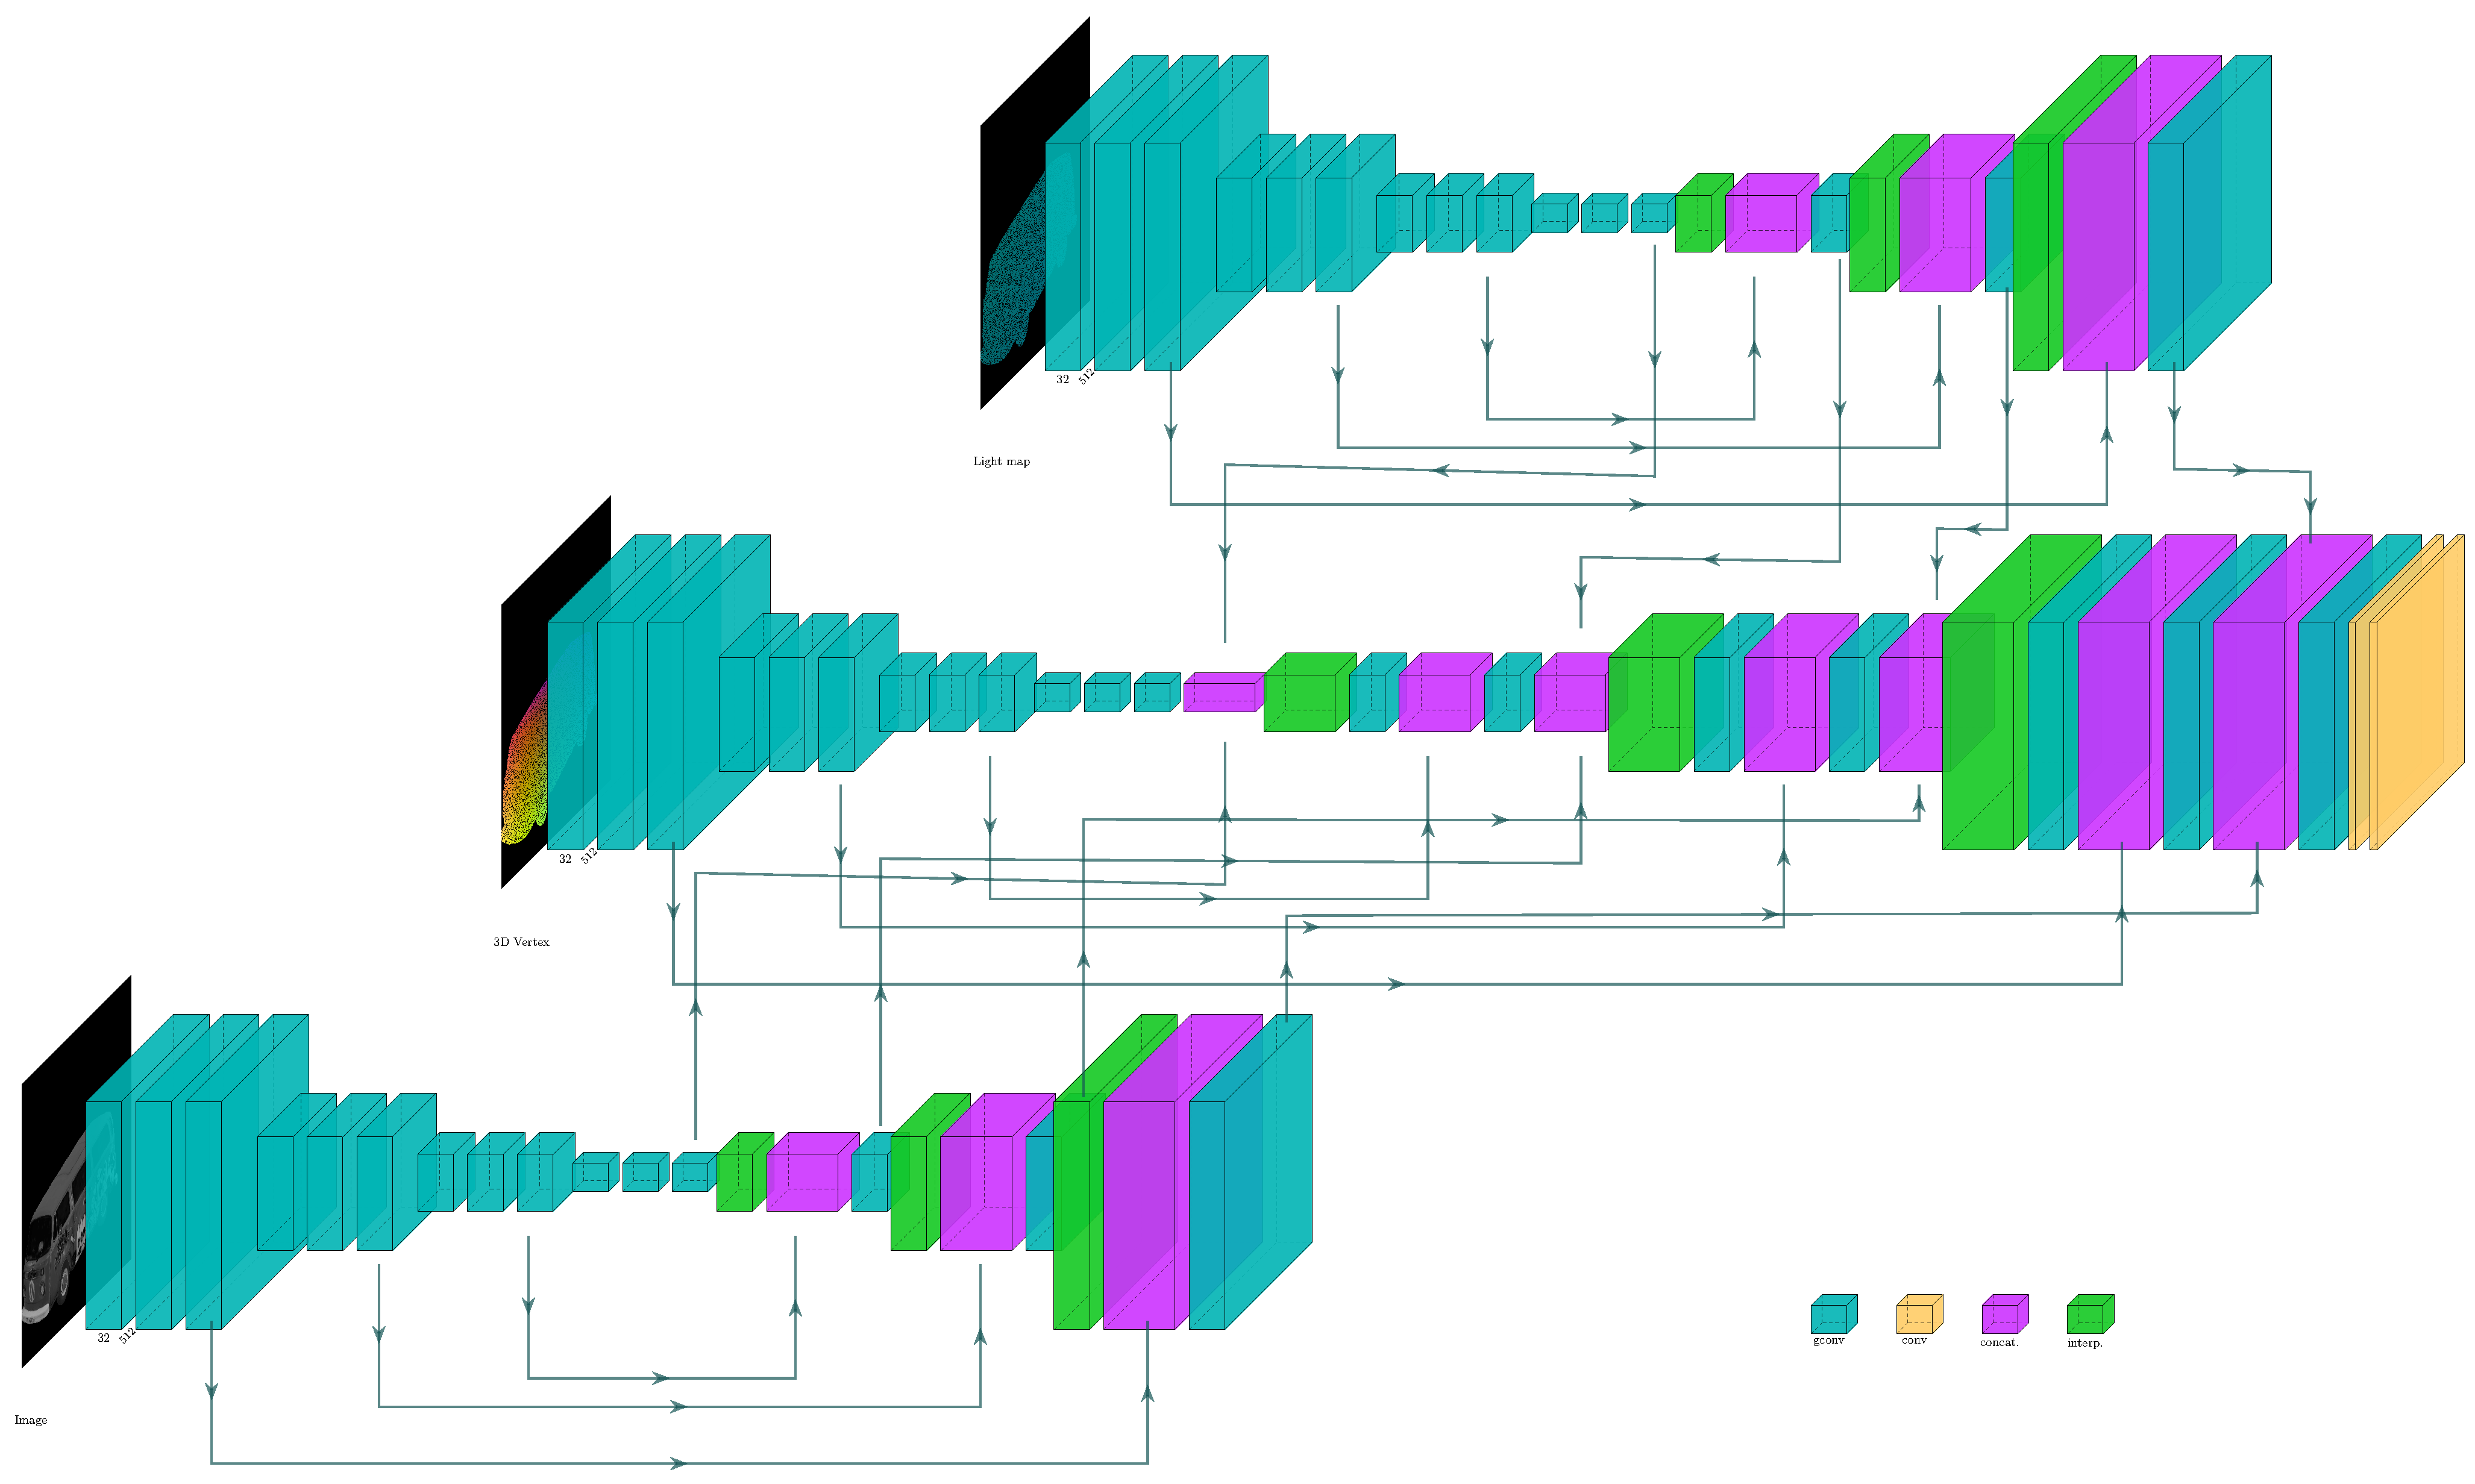
\includegraphics[width=1\textwidth]{Figures/trignet} % Research group name and department name
	\caption{The architecture of TriGNet}
	\label{fig:albedo-gated-archi}
\end{sidewaysfigure}


\subsection{Loss Function}
For the case of normal output, the loss function is the same as Mask-L2 loss as introduced in \ref{par:maskl2}. For the case of the product of albedo and normal, the loss function utilized a scaled Mask-L2 loss, which gives the range of inliers between $ [0,255] $. 



\end{document}
